%pdflatex abra.tex
%convert -density 100x100 abra.pdf abra.png
\documentclass[margin=10pt]{standalone}
\usepackage{tikz}
\usetikzlibrary{arrows.meta, positioning}

\begin{document}
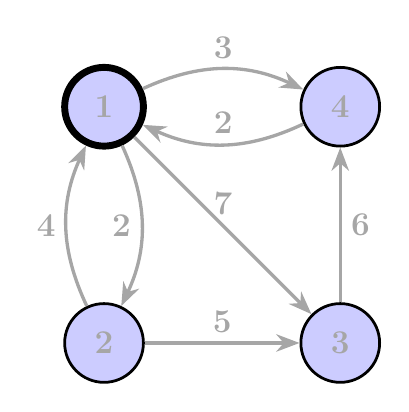
\begin{tikzpicture}[
    planet/.style={circle, draw, minimum size=1cm, fill=blue!20, line width=1pt},
    central/.style={planet, line width=2.5pt},
    edge/.style={->, very thick, >=Stealth, draw=gray!70},
    every edge label/.style={draw=none, font=\bfseries\small, text=gray!70},
    every node/.style={font=\large\bfseries, text=gray!70},
]

% Define planets (nodes)
\node[central] (1) at (0,0) {1};
\node[planet] (2) at (0,-3) {2};
\node[planet] (3) at (3,-3) {3};
\node[planet] (4) at (3,0) {4};

% Edges from example input
\draw[edge] (1) to[bend left=25] node[midway, left, draw=none] {2} (2);
\draw[edge] (2) to[bend left=25] node[midway, left, draw=none] {4} (1);

\draw[edge] (1) -- node[midway, above, draw=none] {7} (3);

\draw[edge] (1) to[bend left=25] node[midway, above, draw=none] {3} (4);
\draw[edge] (4) to[bend left=25] node[midway, above, draw=none] {2} (1);

\draw[edge] (2) -- node[midway, above, draw=none] {5} (3);

\draw[edge] (3) -- node[midway, right, draw=none] {6} (4);

\end{tikzpicture}
\end{document}